\documentclass[10pt, a4paper]{beamer}
\setbeamertemplate{caption}[numbered]


\usetheme{Berkeley}
\usecolortheme{sidebartab}
\usepackage{tabu}
\usepackage{array}
\usepackage{graphicx}
\usepackage{subcaption}
\newcolumntype{P}[1]{>{\centering\arraybackslash}p{#1}}
\begin{document}
	\setbeamertemplate{sidebar left}{}
	\title{Progress Presentation-I}
	\subtitle{e-Yantra Summer Internship-2018 \\ $ $\textbf{Text-to-Image/Video Synthesis using GANs}$ $}
	\author{Aishwarya Kalloli\\Deval Srivastava\\ \vspace{1em}
	Mentors:\\ Aditya Panwar, Kalind Karia}
	\institute{IIT Bombay}
	\date{\today}
	%\addtobeamertemplate{sidebar left}{}{\includegraphics[scale = 0.3]{logowithtext.png}}
	\frame{\titlepage}

\setbeamertemplate{sidebar left}[sidebar theme]
\section{Overview of Project}
\begin{frame}{Overview of Project}
	\begin{itemize}
		\item \textcolor{blue}{Project Name:} Text-to-Image / Video Synthesis using GANs
		\item \textcolor{blue}{Objective:} To generate image or video from given caption
		\item \textcolor{blue}{Deliverables:}
    		\begin{enumerate}
    		    \item To create a model that can generate new images by getting trained on a given dataset
    		    \item Creation of video from these new set of images
    		    \item Prepare proper documentation and tutorial of the solution
    		\end{enumerate}
	\end{itemize}
\end{frame}

\section{Overview of Task}
\begin{frame}{Overview of Task}
\footnotesize{
    \begin{tabular}{|P{1cm}|p{6.2cm}|P{1.7cm}| }
 \hline
 \multicolumn{3}{|c|}{Project Task List} \\
 \hline
 Task & \centering Task & Deadline (days)\\
 \hline
 1 & Understanding the idea and create report on how it can be tackled using Machine Learning: a basic report of 2-5 pages highlighting various algorithms suitable for the task & 2\\
 \hline
 2 & Installing the required software & 1  \\
 \hline
 3 & 
Perform a basic experiment to understand GANs (MNIST)
& 2 \\
 \hline
 4 & Gather the required data-set to train the model & 1-2 \\
 \hline
 5 & Design the model, test its feasibility
 & 2 \\
 \hline
 6 &   
Train the model and calculate the accuracy of the model
  & 6 \\
 \hline
 7 & 
Generate new data-set of images/scenes from the text
  & 4 \\
 \hline
 8 & 
Create a video/scene from the set of generated images
  & 6\\
 \hline
 9 & 
Develop proper tutorial and documentation (with video demo) on the implementation & 4\\
 \hline
 10 & 
Text to audio/music generation (optional)
& 3 \\
\hline
\end{tabular}

%------------
	}
\end{frame}

\section{Task Accomplished}
\begin{frame}{Task Accomplished: Report}
	\begin{itemize}
	\item
{\textcolor{blue}{Understanding the idea and create report on how it can be tackled using Machine Learning.}\linebreak \linebreak
We went through several papers and researched  about different GANs, based on that we decided to use DCGAN that will be conditioned on text embeddings generated by a Character RNN to Generate Images from text
}

\begin{figure}
  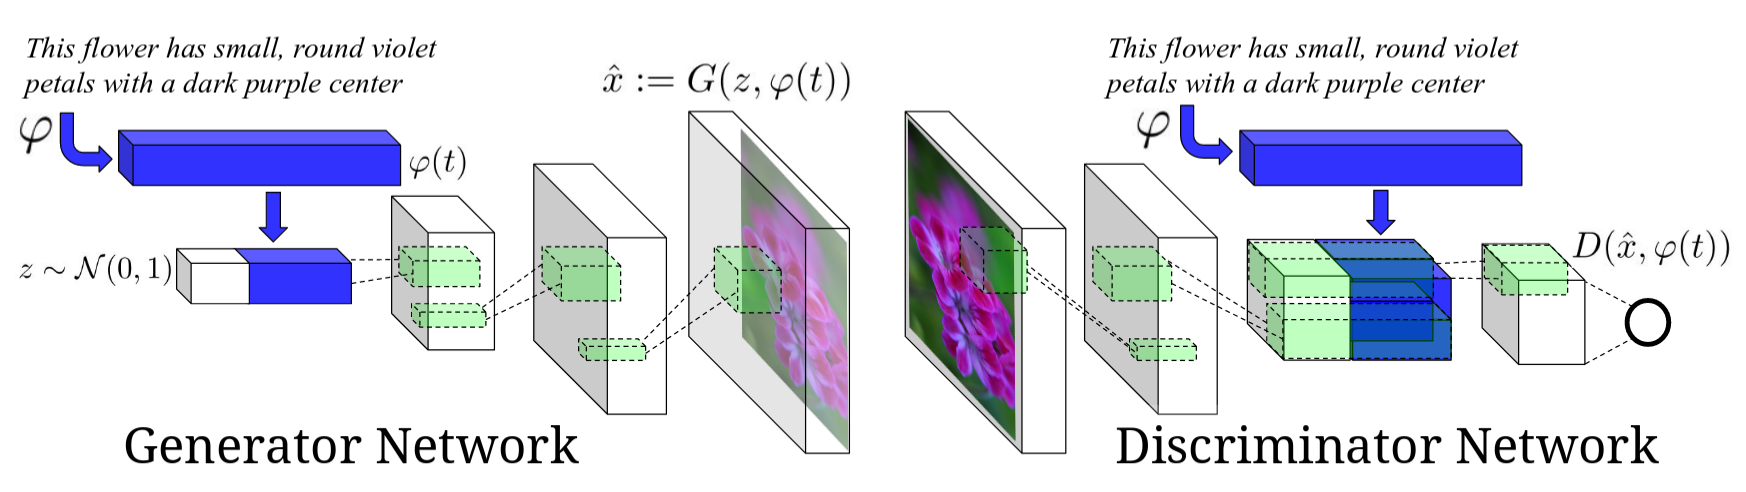
\includegraphics[width=\linewidth]{architecture.png}
  \caption{Architecture\textsuperscript{[1]}}
  \label{fig:architecture}
\end{figure}
% \item
% Perform a basic experiment to understand GANs (MNIST)
% \item 
% Gather the required data-set to train the model
% \item Design the model
{\scriptsize{[1] Generative Adversarial Text to Image Synthesis by Scott Reed, Zeynep Akata, Xinchen Yan, Lajanugen Logeswaran, Bernt Schiele, Honglak Lee}}
	\end{itemize}
\end{frame}

\begin{frame}{Task Accomplished: Software Installation}
	\begin{itemize}
\item {
\textcolor{blue}{Installing the required software}\linebreak 
\begin{enumerate}
    \item Python, PyTorch and Torchvision were successfully installed
    \item A Nvidia GTX 1080Ti was employed for training
    \item CudaNN and Nvidia drivers were installed to allow training models on the GPU
\end{enumerate}

}


% 		\item 
% Installing the required software.
% \item 
% Perform a basic experiment to understand GANs (MNIST)
% \item 
% Gather the required data-set to train the model
% \item Design the model

	\end{itemize}
\end{frame}


\begin{frame}{Task Accomplished: DCGAN}
    \begin{figure}
  \includegraphics[width=\linewidth]{GAN.png}
  \caption{DCGAN block diagram\textsuperscript{[2]}}
%   \caption{DCGAN architecture}
  \label{fig:DCGAN}
\end{figure}
{\scriptsize{[2] GANs from Scratch - Part 1 on Medium}}

\end{frame}

\begin{frame}{Task Accomplished: MNIST example}
	\begin{itemize}
	\item
{\textcolor{blue}{Perform a basic experiment to understand GANs (MNIST)}
\linebreak \linebreak
We used DCGAN to implement the task of generating new images from original MNIST dataset}

\begin{figure}[h!]
  \centering
  \begin{subfigure}[b]{0.4\linewidth}
    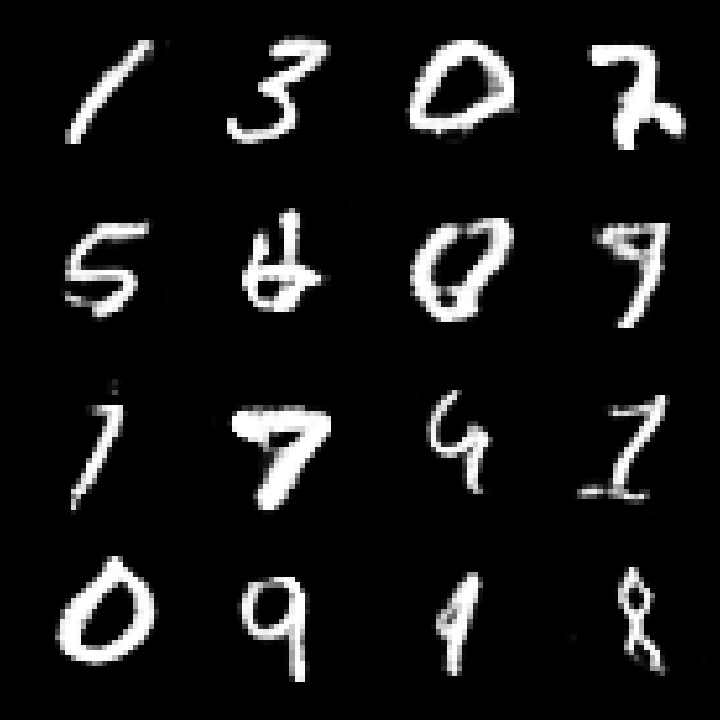
\includegraphics[width=\linewidth]{mnist_ideal.png}
    \caption{original MNIST}
  \end{subfigure}
  \begin{subfigure}[b]{0.407\linewidth}
    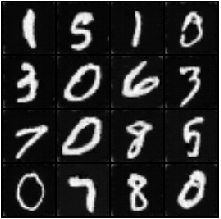
\includegraphics[width=\linewidth]{mnist.png}
    \caption{generated MNIST}
  \end{subfigure}
  \caption{Comparison of generated MNIST images}
  \label{fig:MNIST}
\end{figure}

% \item 
% Perform a basic experiment to understand GANs (MNIST)
% \item 
% Gather the required data-set to train the model
% \item Design the model

	\end{itemize}
\end{frame}





\begin{frame}{Task Accomplished: Gather Dataset}
	\begin{itemize}
	\item
{\textcolor{blue}{Gather the required data-set to train the model for the final solution}
\linebreak \linebreak
We are planning to use COCO image dataset to train out text to image model. COCO is a large-scale object detection, segmentation, and captioning dataset. The dataset has been downloaded and prepared successfully.}

\begin{figure}
  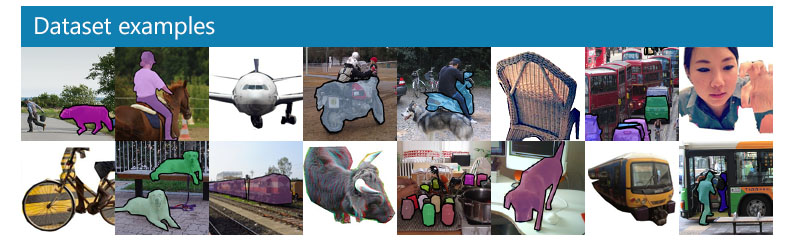
\includegraphics[width=\linewidth]{coco.jpg}
  \caption{COCO Examples.\textsuperscript{[3]}}
  \label{fig:architecture}
\end{figure}
% \item 
% Perform a basic experiment to understand GANs (MNIST)
% \item 
% Gather the required data-set to train the model
% \item Design the model
\linebreak
{\scriptsize{[3] mscoco.org/dataset}}
	\end{itemize}
\end{frame}


\begin{frame}{Task Accomplished: Model Design}
    \begin{itemize}
        \item 
        {\textcolor{blue}{Design the model and test its feasibilty}}
        \linebreak\linebreak
        Designing of model for generating images from text has has been completed but we are yet to test its feasibility and effectiveness. This current model incorporates the standard DCGAN architecture with conditioning on character data.
    \end{itemize}
\end{frame}




\section{Challenges Faced}
\begin{frame}{Challenges Faced}
	\begin{itemize}

		\item Lack of knowledge about PyTorch before starting the internship
		\item Choosing hyper-parameters for GAN leading to efficient convergence
		\item Since GAN is fairly new and is still being actively researched, it took time to find the right algorithm for the task
		\item Finding a right Dataset for the task with captions and creating a dataloader for the same
	\end{itemize}
\end{frame}

\section{Future Plans}
\begin{frame}{Future Plans}
	\begin{itemize}
		\item Test feasibility and effectiveness of our current model
		\item Train the model and calculate the accuracy of the model
		\item Generate new data-set of images/scenes from the text
		\item Next we plan to use these recent images to generate videos by either using a LSTM network to predict the next frame or a Temporal GAN


	\end{itemize}
\end{frame}


\section{Thank You}
\begin{frame}{Thank You}
	\centering THANK YOU !!!
\end{frame}
\end{document}
